%!TEX program = xelatex
\documentclass[10pt,mathserif]{beamer}%,aspectratio=169 %画面比例16:9%
\usepackage{ctex}
\usepackage{xeCJK}
\usepackage{listings}
\usepackage{makecell}
\usepackage{setspace}
\usepackage{array}
\usepackage{booktabs} %调整表格线与上下内容的间隔
\usepackage{subcaption}
\usepackage[slide,algoruled]{algorithm2e}
\usepackage{indentfirst}
\usepackage{multirow}
\usepackage{ulem}
\usepackage{microtype}
\usepackage{caption}
\usepackage{fontspec}
\usepackage{xcolor}
\setmainfont{Times New Roman}
\definecolor{ForestGreen}{RGB}{34,139,34}
\definecolor{BrickRed}{RGB}{182,50,28}
\definecolor{OliveGreen}{RGB}{60,128,49}
\definecolor{CadetBlue}{RGB}{116,114,154}
\definecolor{YellowGreen}{RGB}{152,204,112}
\definecolor{DarkerOrange}{RGB}{200,100,0}
\definecolor{myblue1}{RGB}{70,130,180}

\definecolor{codegreen}{rgb}{0,0.5,0}
\definecolor{codered}{rgb}{0.7,0.1,0.1}
\definecolor{codegray}{rgb}{0.5,0.5,0.5}
\definecolor{codepurple}{rgb}{0.58,0,0.82}
\definecolor{backcolour}{rgb}{1,1,1}
\newcommand{\newDream}[1]{{\color{codepurple} #1}}
\newcommand{\newpid}[1]{{\color{codegreen} #1}}


\usetheme[
	sidebar, % 会在每页左侧加上导航栏,参考 The AAU Sidebar Beamer Theme 设置
	xdblue, % 不选会默认西电红色调,选上会将主题设置为西电蓝色调
	% english % 选上,会将图表等标题还原回英文标题
 ]{XDUstyle}


\title{无人机智能避障与导航}
\institute[北京航空航天大学\\计算机学院]{北京航空航天大学计算机学院23级硕士研究
生} % 中括号部分为导航栏底所用尽可能精简
\author{黄栋篪}
\date{\today}% 时间可自行设置


\setlength{\footnotesep}{0pt}
\setbeamerfont{footnote mark}{size=\tiny}
\setbeamerfont{footnote text}{size=\tiny}
\setbeamertemplate{footnote}{%
  {\setlength{\hsize}{330pt}%
   \usebeamercolor[fg]{footnote mark}%
   \usebeamerfont*{footnote mark}%
   \hspace*{1.5em}%
   \@thefnmark.~%
   \usebeamercolor[fg]{footnote text}%
   \usebeamerfont*{footnote text}%
   \insertfootnotetext\par}}
\setbeamertemplate{bibliography entry article}{}
\setbeamertemplate{bibliography entry title}{}
\setbeamertemplate{bibliography entry location}{}
\setbeamertemplate{bibliography entry note}{}
\setbeamertemplate{navigation symbols}{}
\def\beamer@newblock{%
  \usebeamercolor[fg]{bibliography entry author}%
  \usebeamerfont{bibliography entry author}%
  \usebeamertemplate{bibliography entry author}%
  \def\newblock{%
    \usebeamercolor[fg]{bibliography entry title}%
    \usebeamerfont{bibliography entry title}%
    \usebeamertemplate{bibliography entry title}%
    \def\newblock{%
      \usebeamercolor[fg]{bibliography entry location}%
      \usebeamerfont{bibliography entry location}%
      \usebeamertemplate{bibliography entry location}%
      \def\newblock{%
        \usebeamercolor[fg]{bibliography entry note}%
        \usebeamerfont{bibliography entry note}%
        \usebeamertemplate{bibliography entry note}}}}}
\makeatother
	
\begin{document}

{\xdbg \frame[plain,noframenumbering]{\titlepage}}%首页标题页

\section{overview}

\begin{frame}[t, fragile]
	\frametitle{overview}
	% \setlength{\parindent}{2em}
	\begin{spacing}{1.5}
		SafeDreamer Project主要分为两个部分:
		\begin{itemize}
			\item RL算法. SafeDreamer 结合了世界模型、拉格朗日约束和CEEM的
			一种基于安全强化学习的智能导航算法
			\item Safety-Gymnasium. Safety-Gymnasium是一个基于MuJoCo引擎的仿真验证环境,
			主要面向SafeRL算法的智能体仿真验证,它支持单、多智能体;基于OpenGL库,支持丰富的视觉输入;
			高度可定制化;支持多种智能体和任务;并且集成一个SafeRL算法库。
		\end{itemize}
	\end{spacing}
\end{frame}

\section{RL算法}
\begin{frame}[t, fragile]
	\frametitle{SafeDreamer Algorithm}
	% \setlength{\parindent}{2em}
	\begin{spacing}{1.3}
		SafeDreamer是World Model, Lagrangian SafeRL methods和CCEM三种方法的结合,最终取得了良好的效果。
		\begin{itemize}
			\item \textbf{World Model:} World Model 是一种用来记忆和建模环境的神经网络模块,
			在SafeDreamer中使用DreamerV3来作为World Model,其神经网络结构为RSSM.
			\item \textbf{Lagrangian SafeRL methods:} Lagrangian SafeRL methods 是一种通过拉格朗日方法来求解强
			化学习中有约束优化问题的一种方法。在SafeDreamer中使用Lag-aug和PID-Lag来提高模型性能。
			\item \textbf{CCEM:} 约束交叉熵方法(CCEM),在每次迭代中,首先从策略分布中取样,选择一组精英样本策略,
			并使用它们来更新策略分布。精英样本:我们使用约束值对样本策略进行排序,然后选择约束性能最好的策略。
		\end{itemize}
	\end{spacing}
\end{frame}

\subsection{Model Components}

\begin{frame}[t, fragile]
	\frametitle{Model Components}
	\begin{spacing}{1.5}
		SafeDreamer由world models和actor-critic models组成.
		\begin{equation*}
			\begin{split}
			\begin{array}{ll}
			\text {Observation encoder:} & z_t \sim E_\phi\left(z_t \mid h_t, o_t\right) \\ 
			\text {Observation decoder:} & \hat{o}_t \sim O_\phi\left(\hat{o}_t \mid s_t\right) \\
			\text {Reward decoder:} & \hat{r}_t \sim R_\phi\left(\hat{r}_t \mid s_t\right)  \\ 
			\text {Cost decoder:} & \hat{c}_t \sim C_\phi\left(\hat{c}_t \mid s_t\right) \\
			%\text {Continue decoder:} & \hat{u}_t \sim U_\phi\left(\hat{u}_t \mid s_t\right) \\
			\text {Sequence model:} & h_t, \hat{z}_t=S_\phi\left(h_{t-1}, z_{t-1}, a_{t-1}\right) \\
			%\text {Dynamics:} & \hat{z}_t \sim p_\phi\left(\hat{z}_t \mid h_t\right)\\
			\text{Actor:} & a_{t} \sim \pi_{\theta}( a_t\mid s_t)\\
			\text{Reward critic:} & \hat{v}_{r_t} \sim V_{\psi_r}(\hat{v}_{r_t} \mid s_t)\\
			\text{Cost critic:} & \hat{v}_{c_t} \sim V_{\psi_c}(\hat{v}_{c_t} \mid s_t)\\
			\end{array}
			\end{split}
		\label{eq:definition}
		\end{equation*}
		
	\end{spacing}
\end{frame}

\subsection{Preliminaries}
\subsubsection{Dreamer}
\begin{frame}[t, fragile]
  \frametitle{World Model}
   \begin{figure}
\begin{subfigure}{.5\textwidth}
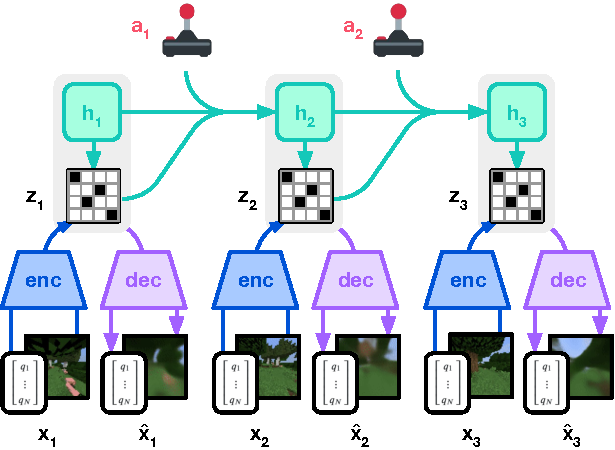
\includegraphics[width=0.75\linewidth]{images/model_wm.pdf}
\caption{World Model Learning}
\end{subfigure}
\begin{subfigure}{.43\textwidth}
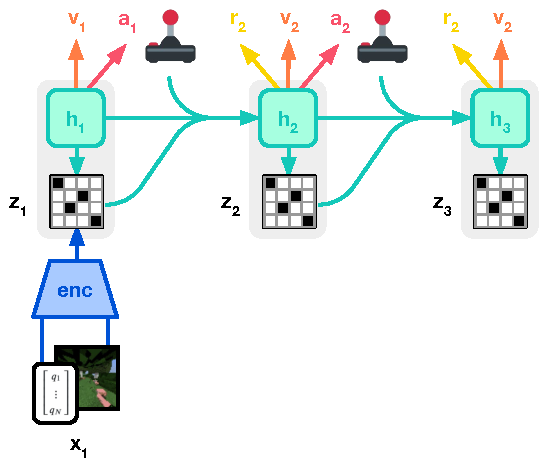
\includegraphics[width=0.75\linewidth]{images/model_ac.pdf}
\caption{Actor Critic Learning}
\end{subfigure}
\label{fig:model}
\end{figure}
{
\fontsize{8pt}{9.6pt}\selectfont
\begin{itemize}
\item \textbf{包含的模型}:SafeDreamer包括世界模型和行动者-评论者模型。
\item \textbf{处理观察和动作}:在每个时间步骤$t$,世界模型接收一个观察$o_t$和一个动作$a_t$,并将观察压缩为一个离散的表示$z_t$。
\item \textbf{预测任务}:这个离散的表示$z_t$,连同动作,被序列模型用来预测下一个表示$\hat{z}_{t+1}$。
\item \textbf{模型状态的定义}:模型状态$s_t=\{h_t, z_t\}$由一个循环状态$h_t$和表示$z_t$的联接表示。
\item \textbf{解码器的作用}:解码器利用模型状态$s_t$预测观察,奖励和代价。
\item \textbf{行动者-评论者模型的输入}:模型状态$s_t$充当行动者-评论者模型的输入,以预测奖励值$v_{r_t}$,代价值$v_{c_t}$和动作$a_t$。
\end{itemize}
}
\end{frame}

\begin{frame}[fragile]
	\frametitle{Lagrangian-based methods}
	PID 拉格朗日方法是一种广泛应用于约束优化问题的算法。它的学习动态通常会展示振荡和超调,这在保证响应性和牺牲安全性方面是一个挑战。PID 拉格朗日方法利用了 PID 控制器的概念,使用比例、积分和微分这三个成分来平衡和控制学习动态,以优化安全性和效率。
	\begin{algorithm}[H]
		\SetAlgoLined
		\KwIn{Proportional coefficient $K_p$, integral coefficient $K_i$, differential coefficient $K_d$}
		
		Initialize previous integral item: $I^0 \leftarrow 0$\;
		Initialize previous episode cost: $J_C^0 \leftarrow 0$\;
		\While{iteration $k$ continues}{
			Receive cost $J_C^k$\;
			$P \leftarrow J_C^k-d$\;
			$D \leftarrow max(0, J_C^{k}-J_C^{k-1})$\;
			$I^k \leftarrow max(0, I^{k-1}+D)$\;
			$\lambda_p \leftarrow max(0, K_p P+K_i I^k + K_d D)$\;
			Return Lagrangian multiplier $\lambda_p$\;
		}
		\caption{PID Lagrangian}
		\label{alg: pid_lag}
		\end{algorithm}
\end{frame}

\begin{frame}[t, fragile]
	\frametitle{CCEM}
 Constrained Cross-Entropy Method 是一种应用于安全强化学习问题的方法。该方法特点在于,它会显式地跟踪其在满足约束方面的表现。特别是,该方法在有限长度的轨道上定义约束,这是以预期的代价形式表示的。
	\begin{algorithm}[H]
	\SetAlgoLined
	\KwIn{Initial parameters $\theta_0$, initial Lagrange multipliers $\lambda_0$}
	Initialize parameters: $\theta \leftarrow \theta_0$, Lagrange multipliers: $\lambda \leftarrow \lambda_0$\;
	\While{the stop criterion is not met}{
		Generate a set of samples $\mathcal{S}$ under the current model\;
		Compute the utility values $u_s$ and constraint violation $c_s$ for all $s \in \mathcal{S}$\;
		Select a set of "elite" samples $\mathcal{S}_{\text{elite}} = \{s \in \mathcal{S}: u_s \text{ is high and } c_s \text{ is low}\}$\;
		Fit the model parameters $\theta$ with $\mathcal{S}_{\text{elite}}$\;
		Update the Lagrange multipliers $\lambda$ according to $c_s$ and current $\lambda$\;
	}
	\caption{Constrained Cross-Entropy Method}
	\end{algorithm}
	\end{frame}

\subsection{Architecture}
\begin{frame}[t, fragile]
	\frametitle{Architecture}
	\begin{figure}
		\centering
		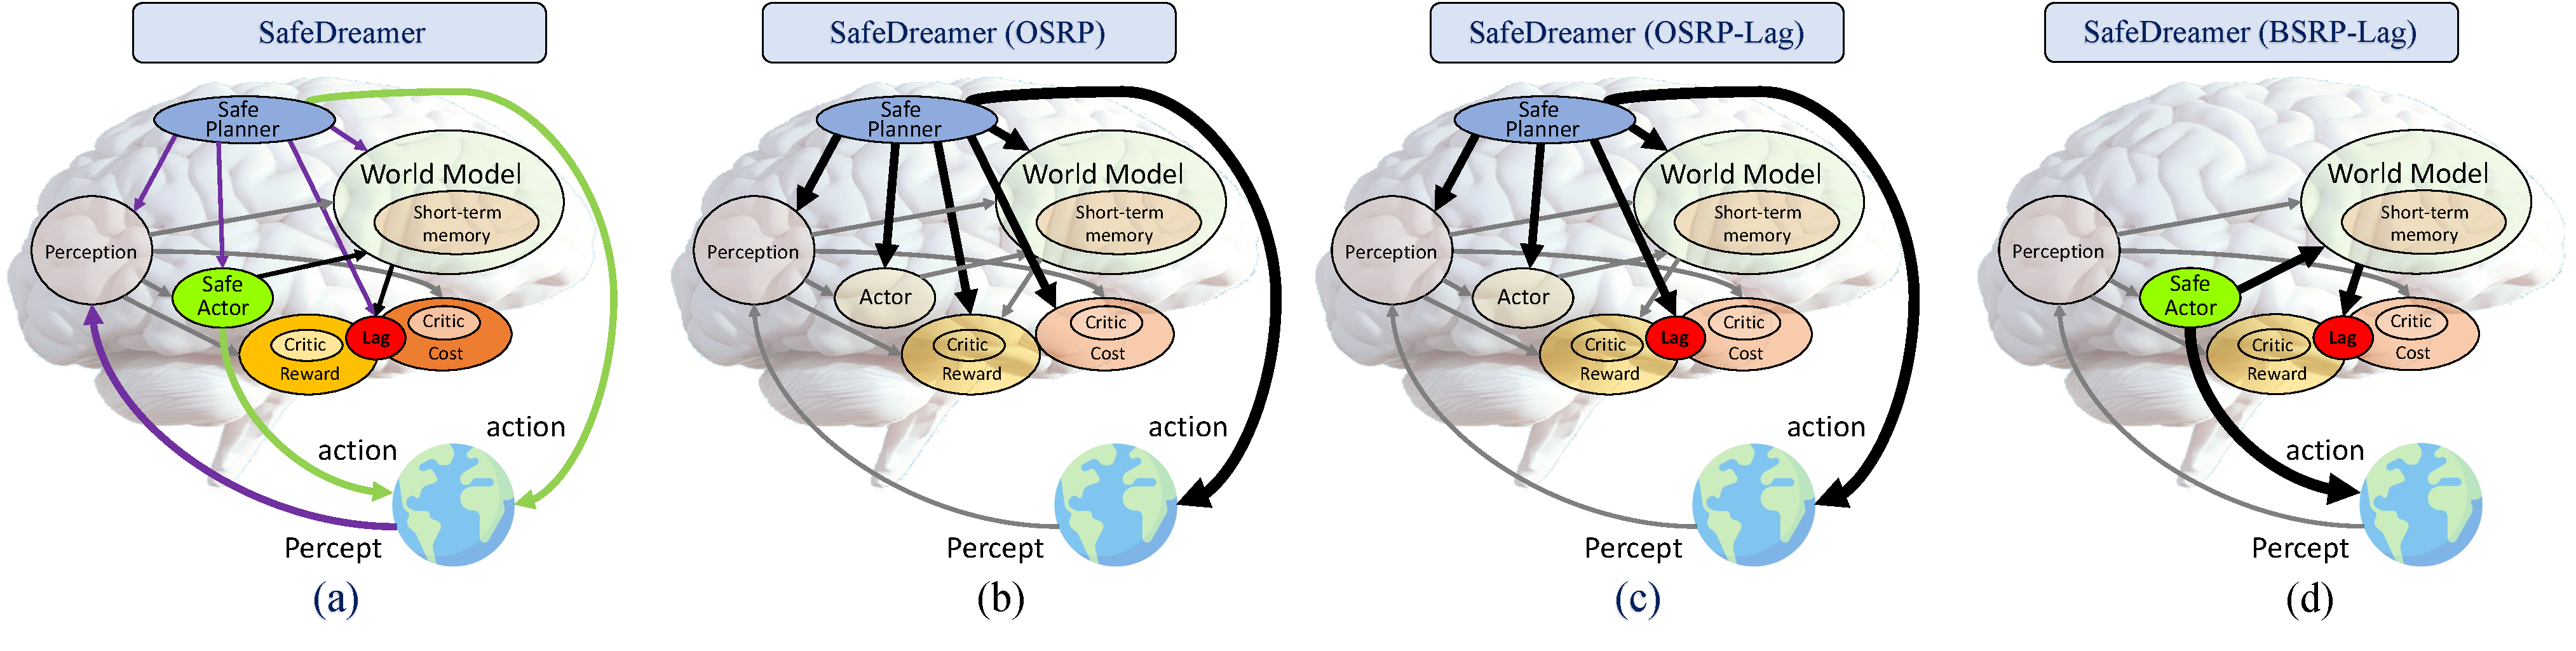
\includegraphics[width=0.9\linewidth]{./images/brain.pdf}
		\caption{SafeDreamer Architecture}
		\label{Fig:net}
	\end{figure}
	\begin{spacing}{1.5}
		OSPR和BSPR是SafeDreamer中的两种实现方式:
		{
		\fontsize{10}\selectfont
		\begin{itemize}
			\item\textbf{OSPR:} 每个决策时间点$t$都会进行在线规划过程,
			该过程会在世界模型中从当前状态$s_{t}$生成状态-动作轨迹。
			每个轨迹都会通过学习到的奖励和代价模型以及它们的评价者进行评估,
			从中选出最优的安全动作轨迹在环境中执行。
			\item\textbf{BSPR:} 在执行者训练期间,
			我们在后台的世界模型中产生长度为$T$=15的想象的隐层表征。
			我们从重播缓冲区的观察开始,从执行者中采样动作,
			并从世界模型中获取观察结果。
		\end{itemize}
		}	
	\end{spacing}
\end{frame}

% \begin{frame}[t, fragile]
% 	\frametitle{OSPR}
% 	\begin{minipage}[t]{0.40\linewidth}
%  {
%  \fontsize{6pt}{7.2pt}\selectfont
% 	定义与概述\begin{itemize}\item 我们引入了在线安全奖励规划 (OSRP),在世界模型中从当前状态生成状态-动作路径,通过学习的奖励和代价模型进行评估。\end{itemize}
% 所采用的方法\begin{itemize}\item 我们采用约束交叉熵方法 (CCEM) 进行规划,初始化一个覆盖规划时域长度的动作均值和标准差序列。\end{itemize}
% 计算过程\begin{itemize}\item 我们使用当前动作分布在世界模型中采样状态路径,并估算每个路径的奖励返回和代价返回。\item 使用代价模型计算一定步数内的总代价。\end{itemize}
% 评估与选择\begin{itemize}\item 我们设定一个轨迹满足代价阈值的准则,并期望得到安全的轨迹。\item 如果安全轨迹的数量小于期望值,我们将采样的动作轨迹全集作为候选动作集;否则,将安全动作轨迹集作为候选动作集。\end{itemize}
% 结果处理\begin{itemize}\item 我们选择排序键值最高的前几个动作轨迹作为精英动作。\item 得到一组新的参数,并在规划过程中使用。\item 从最终分布中采样一个动作轨迹,然后在真实环境中执行这个轨迹的第一个动作。\end{itemize}
% }
% 	\end{minipage}\hfill
% 	\begin{minipage}[t]{0.60\linewidth}
% 	\begin{algorithm}[H]
% 	\SetAlCapNameFnt{\fontsize{8pt}{9.6pt}\selectfont} 
% 	\SetAlCapFnt{\fontsize{8pt}{9.6pt}\selectfont}
% 	\fontsize{8pt}{9.6pt}\selectfont
% 	\DontPrintSemicolon
% 	\SetNoFillComment
% 	\SetAlgoLined
% 	\textbf{Input:} current model state $s_{t}$, planning horizon $H$,\\
% 	num sample/policy/safe trajectories $N_{\pi_\mathcal{N}}, N_{\pi_\theta}, N_{s}$,\\
% 	Lagrangian multiplier $\lambda_p$, cost limit $b$, $\mu^{0}, \sigma^{0}$ for $\mathcal{N}$\\
% 	\For{$j \gets 1 $ \KwTo J}{
% 	   Init. empty safe/candidate/elite actions set $A_s, A_c, A_e$\\
% 	   Sample $N_{\pi_{\mathcal{N}}}+N_{\pi_\theta}$ traj. $\{ s_{i}, a_{i}, s_{i+1}\}_{i=t}^{t+H}$ using $\mathcal{N}(\mu^{j-1}, (\sigma^{j-1})^{2}\mathrm{I})$, $\pi_{\theta}$ within $S_{\phi}$ with  $s_t$ as the initial state\\
% 	   Select the top-k action trajectories with highest $\Omega$ values among $A_c$ as elite actions $A_e$\\
% 	   $\mu^j, \sigma^j = \mathrm{MEAN}\left(A_e\right), \mathrm{STD}\left(A_e\right)$ 
% 	}
% 	\textbf{Return: } $a \sim \mathcal{N}(\mu^{J}, (\sigma^{J})^{2} \mathrm{I})$
% 	\caption{Online Safety-Reward Planning.}
% 	\label{alg:planning}
% 	\end{algorithm}
% 	\end{minipage}
% 	\end{frame}

\begin{frame}[t, fragile]
\frametitle{在线安全奖励规划 (OSPR)}
\begin{columns}[c]
\begin{column}{0.45\textwidth}

\vspace{-1cm}

{\fontsize{6pt}{7.2pt}\selectfont\textbf{定义与概述}
\begin{itemize}
\item 引入在线安全奖励规划 (OSRP),在世界模型中生成状态-动作路径,并通过奖励和代价模型进行评估。
\end{itemize}
    \textbf{方法}\\
    \begin{itemize}
      \item 采用约束交叉熵方法(CCEM)进行规划,初始化一个动作均值和标准差序列。
    \end{itemize}

    \textbf{计算过程}\\
    \begin{itemize}
      \item 使用当前动作分布采样状态路径,并估算每个路径的奖励和代价返回。
      \item 利用代价模型计算一定步数内的总代价。
    \end{itemize}

    \textbf{评估与选择}\\
    \begin{itemize}
      \item 设定轨迹满足代价阈值的准则,期望得到安全的轨迹。
      \item 根据满足条件的轨迹数量,选择候选动作集。
    \end{itemize}
    
    \textbf{结果处理}\\
    \begin{itemize}
      \item 选取排序键值最高的动作轨迹为精英动作。
      \item 得到新的参数组并在规划过程中使用。
      \item 从最终分布中采样动作轨迹,并执行此轨迹的第一个动作。
    \end{itemize}
  }
\end{column}

\begin{column}{0.55\textwidth}
    \begin{spacing}{1.5}
   
    \begin{algorithm}[H]
    \SetAlCapNameFnt{\fontsize{6pt}{8pt}\selectfont} 
    \SetAlCapFnt{\fontsize{6pt}{8pt}\selectfont}
    \fontsize{6pt}{8pt}\selectfont
    \DontPrintSemicolon
    \SetNoFillComment
    \SetAlgoLined
    \caption{在线安全奖励规划}
    \textbf{输入}: 当前模型状态 $s_{t}$, 规划时域 $H$,轨迹样本数 $N_{\pi_\mathcal{N}}, N_{\pi_\theta}, N_{s}$,Lagrangian 乘数 $\lambda_p$,代价限制 $b$,初始 $\mu^{0}, \sigma^{0}$
    
    \For{$j \gets 1$ \KwTo $J$}{
        初始化空的安全/候选/精英动作集 $A_s, A_c, A_e$\\
        在模型中选择 $N_{\pi_{\mathcal{N}}}+N_{\pi_\theta}$ 个轨迹 $\{ s_{i}, a_{i}, s_{i+1}\}_{i=t}^{t+H}$ 使用 $\mathcal{N}(\mu^{j-1}, (\sigma^{j-1})^{2}\mathrm{I})$, $\pi_{\theta}$ 并设 $s_t$ 为起始状态\\
        
        计算并返回每条轨迹的代价以及满足阈值的轨迹集合($N_{\pi_{\mathcal{N}}}+N_{\pi_\theta}$ 轨迹集合, $\gamma$, $C_\phi$, $L$)\\
        判断轨迹集合的大小,选择 $\Omega$ 并确定 $A_c$\\
        从 $A_c$ 中选择 $\Omega$ 值最高的前k个动作轨迹作为精英动作 $A_e$\\
         $\mu^j, \sigma^j = \mathrm{MEAN}\left(A_e\right), \mathrm{STD}\left(A_e\right)$\;
    }
   \textbf{Return: } $a \sim \mathcal{N}(\mu^{J}, (\sigma^{J})^{2} \mathrm{I})$
	\label{alg:planning}
	\end{algorithm}
      
    \end{spacing}
\end{column}
\end{columns}
\end{frame}

\begin{frame}[t, fragile]
	\frametitle{后台安全奖励规划 (BSRP)}
 \begin{columns}[c]
	\begin{column}[t]{0.40\linewidth}
 {
 \vspace{-4cm}
 \begin{spacing}{1.3}
 \fontsize{7pt}{8.4pt}\selectfont
    \begin{itemize}
    \item 使用 Lagrangian 方法进行后台安全奖励规划 (BSRP) 以训练安全 actor。 
    \item 在 actor 训练期间,我们在后台世界模型中生成长度为 $T = 15$ 的假想潜在轨迹。
    \item 我们从回放缓冲区开始观察,从 actor 中采样动作,并从世界模型中采样观察结果。世界模型还预测了奖励和代价,从中我们计算 TD($\lambda$) 值 $R^\lambda(s_t)$ 和 $C^\lambda(s_t)$。
    \item 这些值被用于随机反向传播,以更新安全 actor。
    \item 在此过程中的训练损失指导了安全 actor 去最大化期望回报和熵,同时最小化代价回报,利用了增强的拉格朗日方法。
    \end{itemize}
     \end{spacing}
}
	\end{column}
	\begin{column}[t]{0.60\linewidth}
	\begin{algorithm}[H]
	\SetAlCapNameFnt{\fontsize{6pt}{7.2pt}\selectfont} 
	\SetAlCapFnt{\fontsize{6pt}{7.2pt}\selectfont}
	\fontsize{6pt}{7.2pt}\selectfont
	\DontPrintSemicolon
	\SetNoFillComment
	\SetAlgoLined
\KwIn{批长度 $T$, 批大小 $B$, 事件长度 $L$, 初始拉格朗日乘数 $\lambda_p$}
初始化世界模型参数 $\phi$, 演员-评论家参数 $\theta, V_{\psi_r}, V_{\psi_c}$ \;
用随机策略初始化数据集 $\mathcal{D}$\;
\While{\emph{未收敛}}{
  从 $\mathcal{D}$ 中采样 $B$ 条轨迹 $\{ o_{t}, a_{t}, o_{t+1}, r_{t+1}, c_{t+1}\}_{t:t+T}$ \;
  更新世界模型 \;
  将 $o_{t:t+T}$ 通过世界模型压缩成 $s_{t: t+T}$\;
使用演员在世界模型中生成潜在漫步,以 $s_{t: t+T}$ 为初始状态\;
  更新奖励和代价评论家\;
  \newDream{更新安全演员和 $\lambda_p$} \tcp*{仅限 BSRP}
  $\mathcal{J}_{\mathcal{C}} \leftarrow 0$\;
  \For{$t = 1$ to $L$}{
    通过 ${s}_t \sim S_\phi(o_t, s_{t-1}, a_{t-1})$ 将 $o_t$ 压缩成潜在状态\;
    \newDream{采样 $a_t \sim \pi_a(\cdot | s_t)$}\tcp*{仅限 BSRP}
    \newpid{采样 $a_t \sim Planner(s_t, \lambda_p)$}\tcp*{仅限 OSRP}
    执行动作 $a_t$, 观察环境返回的 $o_{t + 1},r_{t+1}, c_{t+1}$\;
    更新数据集 $\mathcal{D} \leftarrow \mathcal{D} \cup\left\{o_{t}, a_{t}, o_{t+1}, r_{t+1}, c_{t+1}\right\}$\;
    $\mathcal{J}_{\mathcal{C}} \leftarrow \mathcal{J}_{\mathcal{C}} + c_{t+1}$\;
  }
  \newpid{用 $\mathcal{J}_{\mathcal{C}}$ 更新 $\lambda_p$}\tcp*{仅限 OSR}
}
\caption{~~SafeDreamer. \newpid{绿色是 OSRP}, \newDream{紫色是 BSRP}}
\label{alg: train_model_ac}
	\end{algorithm}
	\end{column}
\end{columns}
\end{frame}

\section{Safety-Gymnasium}

\subsection{intro}

\begin{frame}[t, fragile]
\frametitle{Safety-Gymnasium}

\begin{minipage}[t]{\textwidth}
   \textbf{Safety-Gymnasium:} 这是一个专为安全强化学习(SafeRL)构建的仿真环境, 基于 Gymnasium 和 MuJoCo 构建.通过增强现有的 Safety Gym 框架, 支持\textbf{\textcolor{red}{vision-only}}和多智能体任务. 此外, 该项目还集成了 SafePO, 一个单文件风格的算法库, 包含超过 16 种最新的算法。
   
   \vspace{0.3cm}
   
   \textbf{主要组成部分:}

   
   \vspace{0.2cm}
   \hspace*{0.2cm} 
   (1) 智能体模型 \hspace*{1cm} 
   (2) 安全任务 \hspace*{1cm} 
   (3) 安全约束
   \hfill
\end{minipage}

% \begin{minipage}[t]{\textwidth}
% \begin{columns}
% \begin{column}{0.35\textwidth}
%   \textbf{主要组成部分:}
%   \begin{enumerate}
%     \item 智能体模型
%     \item 安全任务
%     \item 安全约束
%   \end{enumerate}
% \end{column}

% \begin{column}{0.65\textwidth}
% \begin{figure}
%   \centering
%   \includegraphics[width=0.95\textwidth]{SafeDreamer/images/task.pdf}
%   \vspace*{-0.5\baselineskip}
%   \setbeamerfont{caption}{size=\tiny}
%   \caption{Tasks from Safety-Gymnasium.}
%   \label{fig:task}
% \end{figure}
% \end{column}
% \end{columns}
% \begin{figure}
%   \centering
%   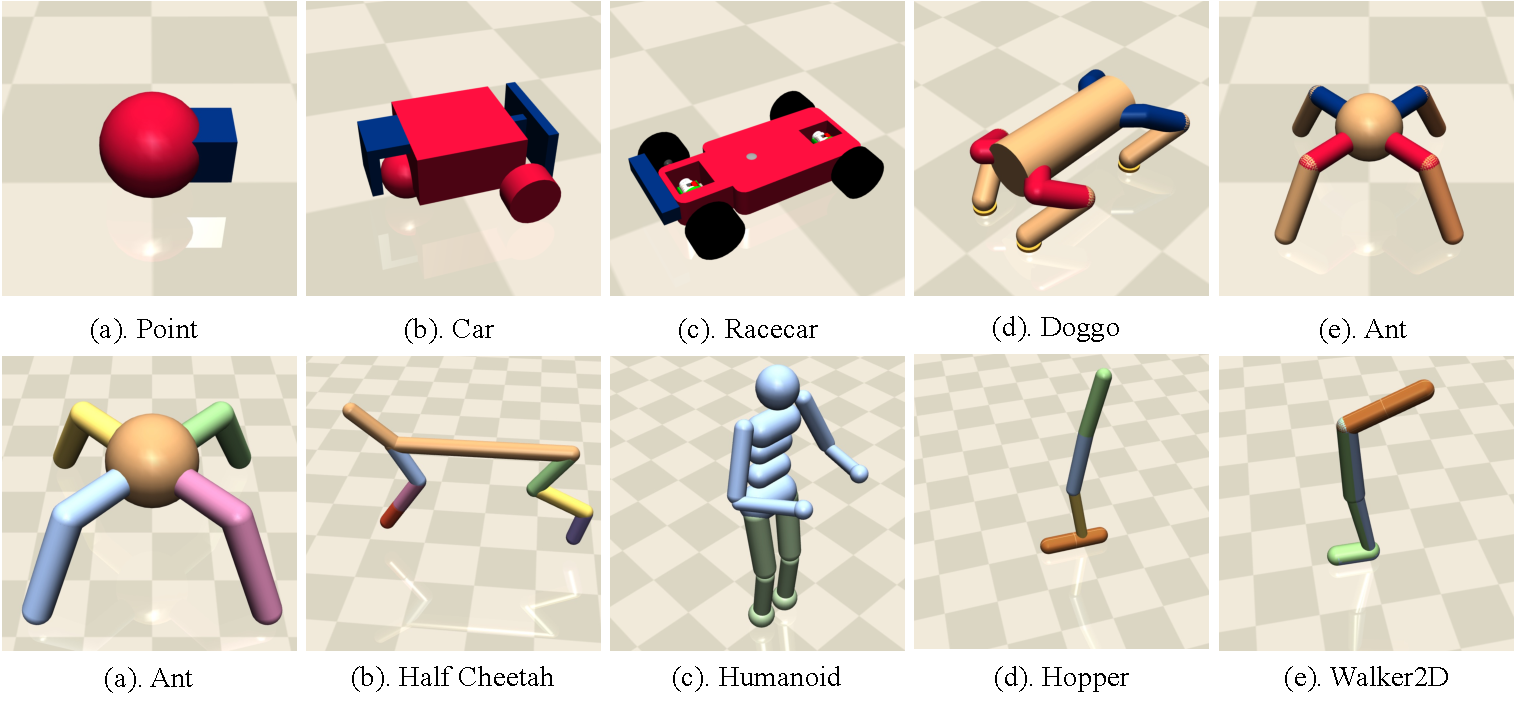
\includegraphics[width=0.8\textwidth]{Safety-Gymnasium/assets/main-paper/agent.pdf}
%   \vspace*{-0.5\baselineskip}
%   \setbeamerfont{caption}{size=\tiny}
%   \caption{Tasks from Safety-Gymnasium.}
%   \label{fig:task}
% \end{figure}
% \end{minipage}
\vfill
\begin{minipage}[bp]{\textwidth}

\begin{figure}
  \centering
  \includegraphics[width=0.95\textwidth]{images/task.pdf}
  \vspace*{-0.8\baselineskip}
  \caption{Tasks from Safety-Gymnasium.}
  \label{fig:task}
\end{figure}

\end{minipage}

\end{frame}
\subsection{Agents}
\begin{frame}[t,fragile]
    \frametitle{智能体模型}
\begin{figure}[ht]
  \centering
  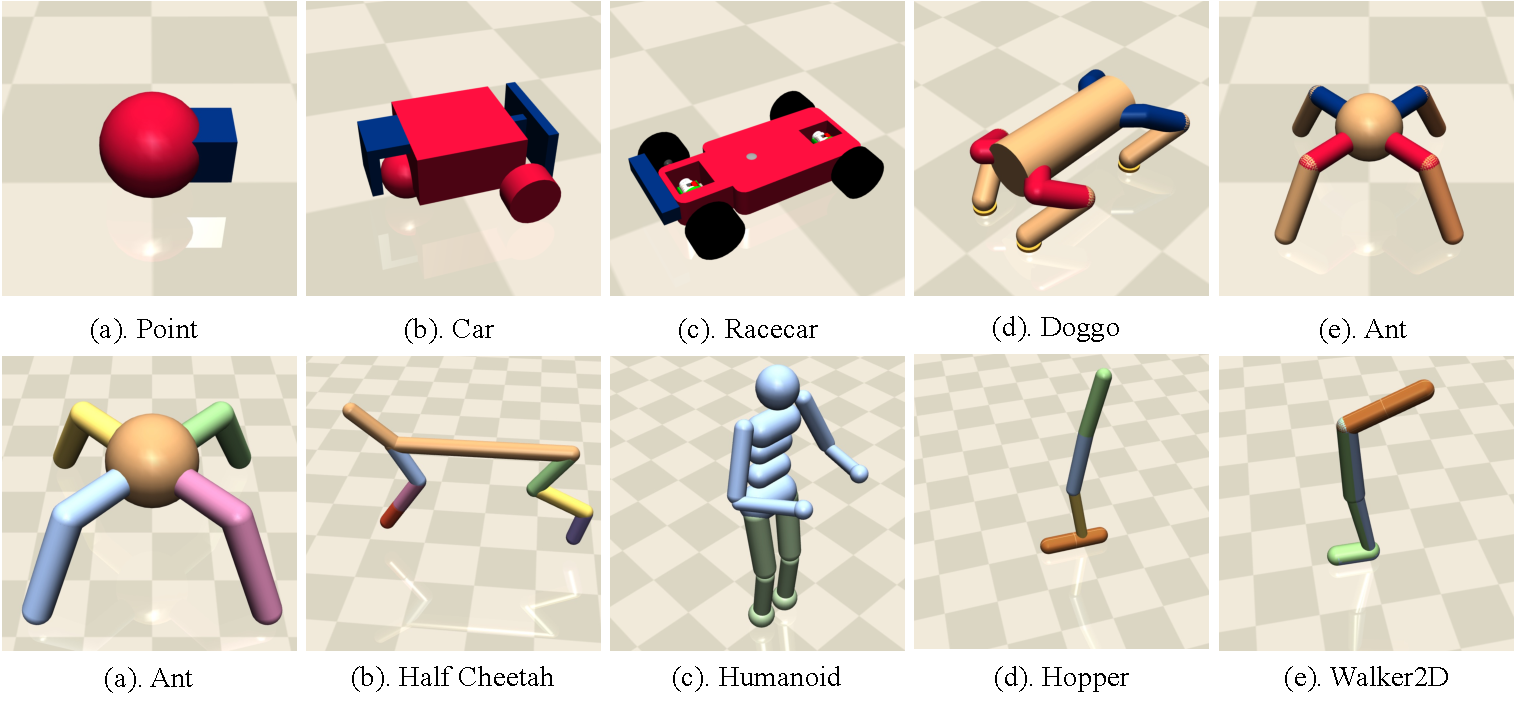
\includegraphics[width=0.9\linewidth]{Safety-Gymnasium/assets/main-paper/agent.pdf}
  \setbeamerfont{caption}{size=\tiny}
  \caption{\textbf{Upper: }The Single-Agent Robots. \textbf{Lower:} The Multi-Agent Robots.}
  \label{pic:agent}
\end{figure}
\vspace{-0.5cm}
\begin{itemize}
{
\fontsize{8pt}{9.6pt}\selectfont
    \item \textbf{预设机器人:} Safety-Gymnasium 继承了 Safety Gym 里的三种现有智能体——Point,Car 和 Doggo。
    \item \textbf{优化改进:} 通过精心调整模型参数,成功地缓解了 Point 和 Car 智能体在运行中过度振荡的问题。
    \item \textbf{新增机器人:} 在此基础上,引入了两种额外的机器人 —— racecar 和 ant,以丰富单智能体场景。
    \item \textbf{多智能体机器人:} 从多智能体 MuJoCo 中借鉴了一些配置,解构了原本的单智能体结构,并使多个智能体可以控制不同的身体部分。
}
\end{itemize}
\end{frame}


\subsection{Tasks}
\begin{frame}[t,fragile]
    \frametitle{安全任务}
\begin{figure}[ht]
  \centering
  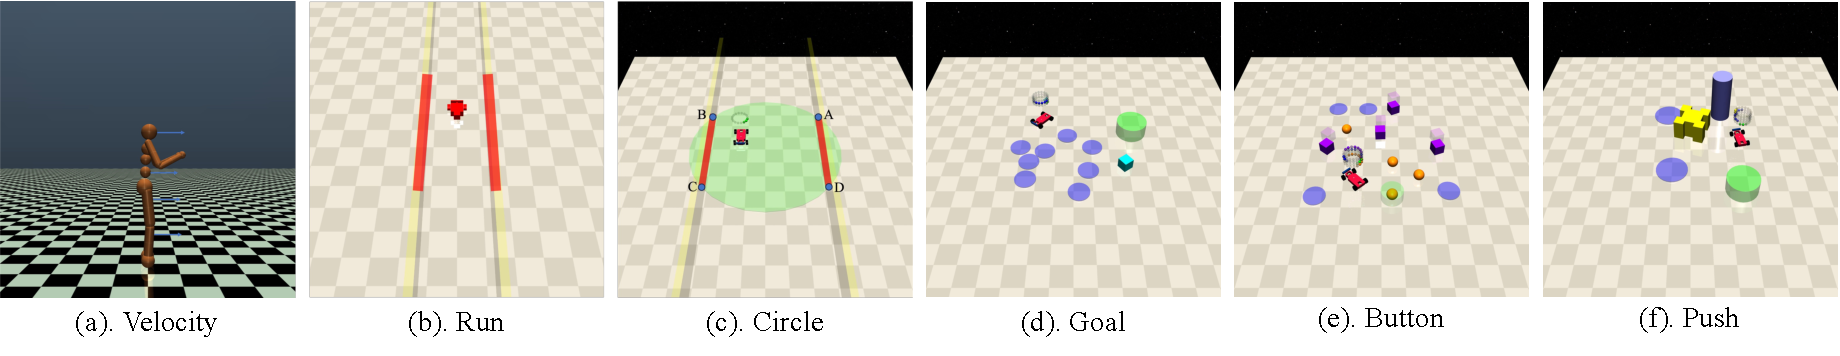
\includegraphics[width=0.9\linewidth]{Safety-Gymnasium/assets/main-paper/tasks.pdf}
  \caption{Tasks of Gymnasium-based Environments}
  \label{pic:agent}
\end{figure}
\vspace{-0.5cm}
\begin{itemize}
{
\fontsize{8pt}{9.6pt}\selectfont
    \item \textbf{Velocity:} 通过对铰链施加扭矩,使机器人在前向(右)方向上协调腿部运动。
    \item \textbf{Run:} 机器人从随机的初始方向和特定的初始速度开始,努力到达地图的另一边。
    \item \textbf{Circle:} 通过沿着绿色圆移动且不能进入红色区域外部来最大化奖励,因此,它的最优路径遵循 AD 和 BC 的线段。
    \item \textbf{Goal:} 机器人导航至多个目标位置。成功到达一个目标后,其位置在保持整体布局不变的情况下随机重置。
    \item \textbf{Push:} 目标是将一个盒子移动到一系列目标位置。与Goal任务类似,每个成就后会生成新的随机目标位置。
    \item \textbf{Button:} 目标是激活环境中分布的一系列目标按钮。智能体的目标是导航至并接触当前突出显示的按钮,称为目标按钮。
}
\end{itemize}
\end{frame}



\subsection{Constraints}
\begin{frame}[t,fragile]
    \frametitle{安全约束}
\begin{figure}[ht]
  \centering
  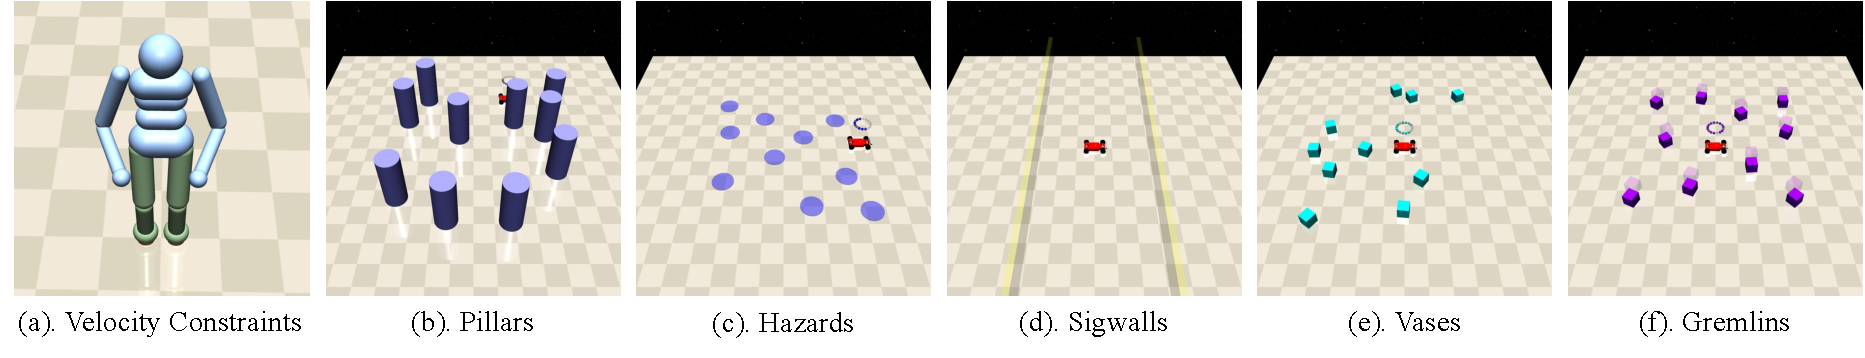
\includegraphics[width=0.9\linewidth]{Safety-Gymnasium/assets/main-paper/constraints.pdf}
  \caption{Constraints of Gymnasium-based Environments}
  \label{pic:agent}
\end{figure}
\vspace{-0.5cm}
\begin{spacing}{1.2}
\begin{itemize}
{
\fontsize{8pt}{9.6pt}\selectfont
    \item \textbf{Velocity-Constraint:} 在这些任务中,智能体通过更快地移动来获得更高的奖励,但也必须遵守速度限制以确保安全。
    \item \textbf{Pillars:} 用于在环境中表示大型圆柱形障碍。在一般情况下,接触柱子会产生代价。
    \item \textbf{Hazards:} 用于模拟环境中的危险区域,对智能体进入这些区域造成代价。
    \item \textbf{Sigwalls:} 开发的特殊用于Circle任务。从安全区内部越过围墙到外部会产生代价。
    \item \textbf{Vases:} 代表环境中的静态和易碎物体。触摸或移动这些物体会对智能体产生代价。
    \item \textbf{Gremlins:} 代表环境中可以与智能体互动的移动物体。
}
\end{itemize}
\end{spacing}
\end{frame}



\subsection{Vision-only tasks}
\begin{frame}[t,fragile]
    \frametitle{Vision-only tasks}
\begin{figure}[ht]
  \centering
  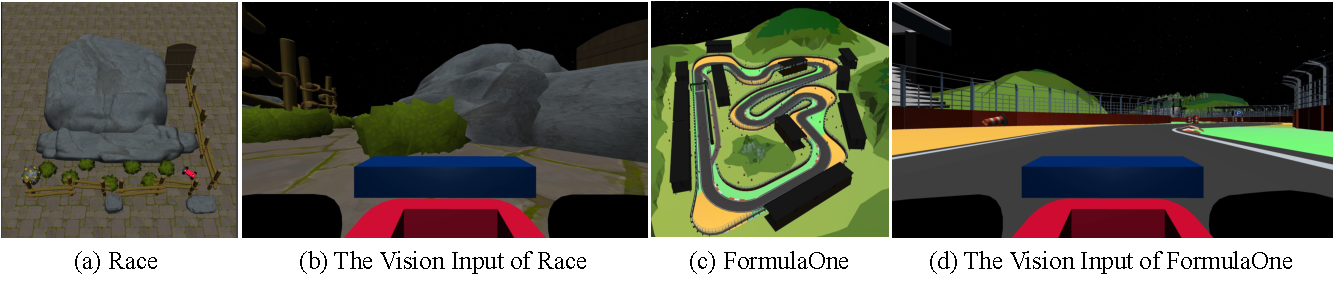
\includegraphics[width=0.9\linewidth]{Safety-Gymnasium/assets/main-paper/vision-task.pdf}
  \caption{Vision-only Tasks of Gymnasium-based Environments.}
  \label{pic:agent}
\end{figure}
\vspace{-0.5cm}
\begin{spacing}{1.2}
原始框架的不足:
\begin{itemize}
{
\fontsize{8pt}{9.6pt}\selectfont
   
    \item \textbf{环境逼真度低:}尽管Safety Gym的初始版本提供了基本的视觉输入支持,但其环境的逼真性有待提高。
Safety Gymnasium的改进:
}
\end{itemize}
Safety Gymnasium的改进:
\begin{itemize}
{
\fontsize{8pt}{9.6pt}\selectfont
   
       \item \textbf{提高环境逼真度:}Safety Gymnasium使用MuJoCo模型制定了一个更真实的视觉环境,增强了环境的逼真性。
    \item \textbf{整合了更多的视觉输入:}相较于原始框架,这个改进版的环境能够整合RGB和RGB-D这两种输入,从而提供了更为准确和全面的视觉信息。
}
\end{itemize}
\end{spacing}
\end{frame}

\subsection{SafePO}
\begin{frame}[t,fragile]

    \frametitle{SafePO}
\begin{figure}[ht]
  \centering
  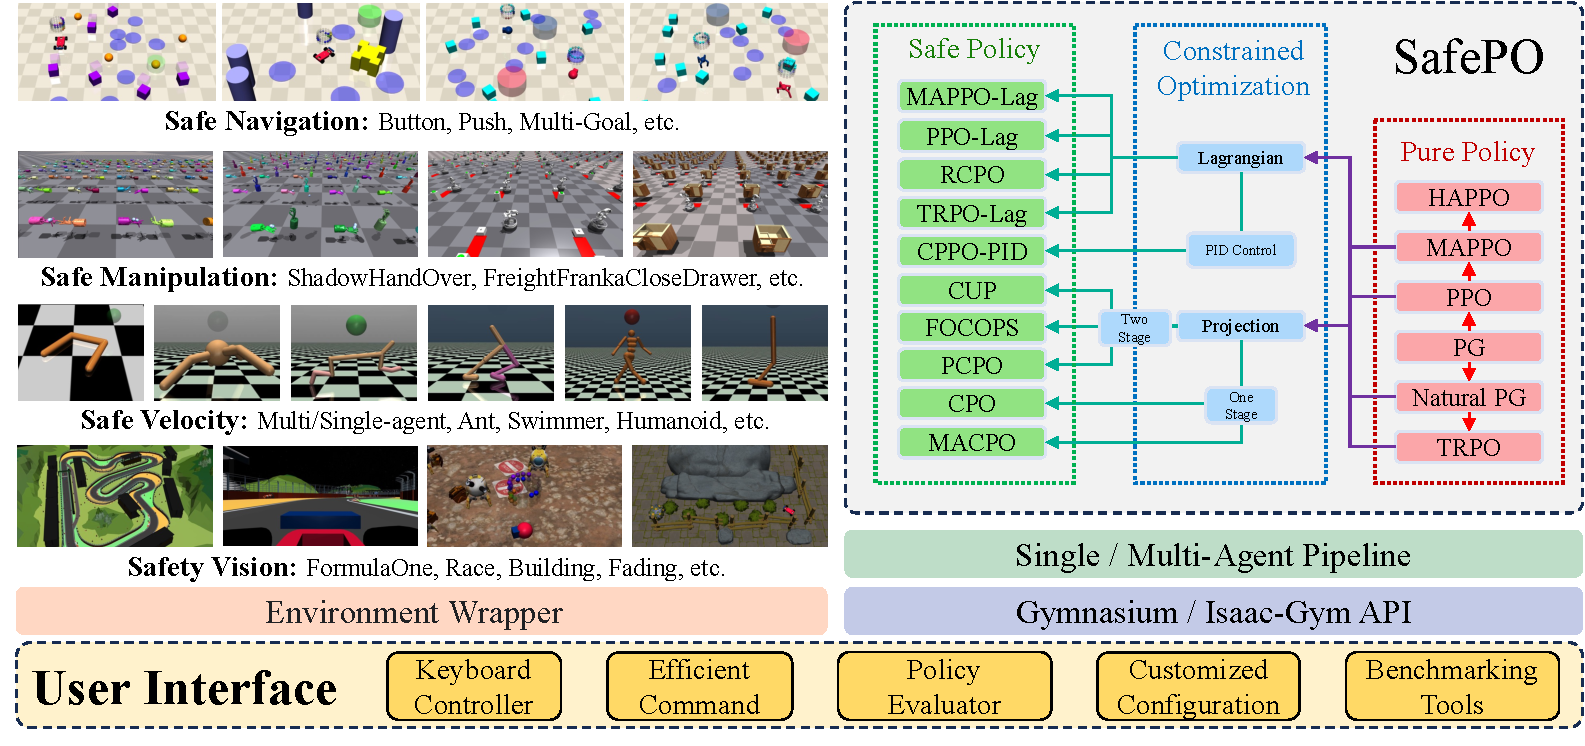
\includegraphics[width=0.8\linewidth]{Safety-Gymnasium/assets/main-paper/arch.pdf}
  \vspace*{-0.5\baselineskip}
  \caption{The Architecture of \texttt{SafePO}}
  \label{pic:architecture}
\end{figure}
\vspace{-0.5cm}
\begin{itemize}
{
\fontsize{8pt}{9.6pt}\selectfont
    \item \textbf{正确性:} SafePO确保了高度的准确性与可靠性,与现有基准相比具备超越或匹敌的性能。
    \item \textbf{可扩展性:} 新算法可以方便地集成到SafePO中,增强其可扩展性。
    \item \textbf{日志记录和可视化:} SafePO支持TensorBoard和WandB,提供了许多参数和结果的可视化,使训练过程透明化。
    \item \textbf{详细的文档指南:} SafePO配有详尽的文档,从安装指南到高级定制都有涵盖,方便用户参考使用。
}
\end{itemize}

\end{frame}


\end{document} 
